\documentclass[main.tex]{subfiles}

\begin{document}
\subsubsection{ASIC/PIO}
ASIC/PIO:ns uppgift är att delegera databussen samt läs- och skrivsignalerna
till rätt port. Data som går till portarna hanteras annorlunda från data som
kommer från portarna. Data som kommer från portarna läses alltid från porten
men läggs endast på databussen när den specifika porten ska läsas ifrån. Å
andra sidan skrivs alltid datan från en buffer till porten men buffern läser
endast från databussen när en skrivning till porten sker. Figur \ref{fig:port}
visar hur varje port är uppbyggd. Läs och skrivsignalerna går endast vidare
till den port som är vald med de fem lägsta bitarna av adressbussen.
Lässignalen \mono{rd} aktiveras vid en \mono{in}-instruktion och \mono{wr}
aktiveras vid en \mono{out}-instruktion. Åtta av tio egentliga portar för TI83p
har implementerats. De portar som saknas hanterar exekveringsmask och
skrivskydd för ROM.

\begin{figure}[H]
    \center
    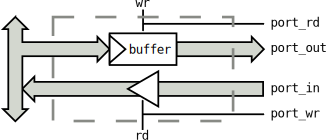
\includegraphics{port.eps}
    \caption{Implementation av en port.}
    \label{fig:port}
\end{figure}

In- och utsignalerna går vidare till de komponenter som hanterar porten, som
kan ses i blockschema \ref{diag:ti}. Flera komponenter kan ta emot data från en
port vid en \mono{out}-instruktion men endast en komponent skriver tillbaka
data vid en \mono{in}-instruktion. Läs och skrivsignalerna skickas även till
komponenterna eftersom vissa reagerar på läsningar och skrivningar. Vissa
portar skickar direkt tillbaka datan från buffern vid en läsning.

I praktiken speglar TI-miniräknaren flera portadresser till en och samma port.
Detta löses genom att aktivera lässignalen och skrivsignalen till
``originalporten'' om någon av spegelbilderna ligger på adressbussen. Eftersom
fem bitar väljer port kan det finnas upp till 32 portar. Egentligen finns
endast tio portar men nästan alla 32 adresser pekar till någon av dessa.
\end{document}
